\documentclass[acmsmall,screen,nonacm]{acmart}

\settopmatter{printfolios=true,printacmref=false}
\renewcommand\footnotetextcopyrightpermission[1]{}
\setcopyright{none}
\usepackage{booktabs}
\usepackage{tabularx}
\usepackage{multirow}
\usepackage{amsmath}
\usepackage{array}
\usepackage{enumitem}
\usepackage{graphicx}
\usepackage{url}
\usepackage{microtype}

\title{Does Prompt Wording Change Scientific Conclusions? A Controlled Study of Prompt Sensitivity in Instruction-Tuned Language Models}

\author{Akula Advaith}
\affiliation{%
  \institution{Indian Institute of Information Technology Allahabad}
  \city{Prayagraj}
  \country{India}}

\begin{document}

\begin{abstract}
Large language models are increasingly used to summarize research evidence, but the conclusion they produce may depend on how a task is worded. This study examines whether short, meaning-preserving paraphrases of a source-only instruction affect the source fidelity and substantive stability of one-sentence scientific conclusions. Eight publisher-checked scientific abstracts were processed under three prompt conditions using two instruction-tuned models from the Qwen2.5 family (0.5B and 1.5B parameters), yielding 48 outputs under greedy decoding. Each output was assessed against its source abstract on central-conclusion fidelity, evidential support, and preservation of scope and qualifications. Prompt pairs were classified as stable, emphasis shift, substantive shift, or contradiction; lexical overlap was measured separately using TF--IDF cosine similarity. In the AI-assisted annotation pass, the mean source-grounded quality score was 0.618 for the 0.5B model and 0.757 for the 1.5B model. Of 48 prompt-pair comparisons, 25 were classified as stable, 15 as emphasis shifts, eight as substantive shifts, and none as contradictions. All eight substantive shifts occurred in the 0.5B condition. Scope and qualification fidelity was the weakest scoring dimension (mean 0.500). These descriptive findings suggest that prompt paraphrases can alter which evidence or qualifications appear in generated conclusions, while lexical similarity alone does not establish substantive stability. The study is limited by its small purposive sample, single greedy generation per condition, same-family model comparison, and AI-assisted rather than independent human annotation.
\end{abstract}

\keywords{prompt sensitivity, large language models, scientific summarization, conclusion stability, source fidelity, TF--IDF, reproducibility}

\maketitle

\section{Introduction}
Large language models (LLMs) are increasingly used to summarize scientific literature, extract evidence, and support research workflows. In these settings, the generated response is not determined by the evidence alone: the instruction that frames the task also shapes what the model is asked to produce. Prior work has documented sensitivity to prompt formulation and prompt ordering, and has developed explicit frameworks for measuring prompt sensitivity \cite{lu2022,zhuo2024,schulhoff2024}. This creates a practical concern for research use. Two instructions can appear to request the same task while eliciting conclusions that differ in their emphasis, scope, or treatment of qualifications.

The distinction between wording variation and conclusion variation is important. Two outputs may use different words yet preserve the same scientific claim. Conversely, outputs with substantial lexical overlap may disagree about the population, conditions, outcome, or limitations described in the source. A lexical metric therefore cannot, by itself, determine whether a conclusion remains faithful to the evidence. ProSA provides a structured approach to prompt-sensitivity measurement and motivates pairwise comparison of outputs, but the present study does not reproduce its benchmark or original PromptSensiScore implementation \cite{zhuo2024}.

This paper investigates a narrower question arising from the preceding literature review: when the same scientific abstract is supplied to a fixed model, do short paraphrases of the instruction change the source fidelity or substantive stability of the one-sentence conclusion? We compare two model sizes from the Qwen2.5 instruction-tuned family and hold the abstract, shared constraints, decoding configuration, and output target constant within each comparison \cite{qwen2024}.

The study addresses two research questions:
\begin{itemize}[leftmargin=*]
  \item \textbf{RQ1:} Under deterministic decoding, how do three meaning-preserving paraphrases of the same source-only instruction affect the source fidelity and substantive stability of one-sentence scientific conclusions generated from the same abstract?
  \item \textbf{RQ2:} How well does lexical similarity between generated conclusions align with source-grounded judgments of substantive stability?
\end{itemize}

The contribution is an exploratory controlled comparison of conclusion-level prompt variation across eight heterogeneous scientific abstracts and two model sizes. The study is not presented as the first investigation of prompt sensitivity, and it does not claim broad generalization from this small sample. Instead, it documents a repeatable protocol, source-grounded assessments, pairwise conclusion relations, and failure cases that illustrate how paraphrased task instructions may affect scientific claim preservation.

\section{Related Work}
\subsection{Prompt sensitivity and paraphrase variation}
Prompt sensitivity refers to changes in model outputs or task performance caused by changes in prompt wording, structure, examples, ordering, or other prompt properties. Prompting surveys describe a wide range of design choices, while empirical studies show that even changes that preserve the intended task can alter model behaviour \cite{schulhoff2024,lu2022}. ProSA introduces PromptSensiScore and examines prompt sensitivity across models and tasks; its findings motivate measuring variation at the instance level rather than relying only on a single prompt template \cite{zhuo2024}.

The current experiment focuses on three short task phrases rather than few-shot demonstrations or complex prompt templates. The prompts request the same output target and share all evidence constraints. This design isolates the intended wording factor more narrowly than a comparison in which instructions, output formats, or evidence inputs also differ. However, semantic equivalence is an experimental assumption, not a guarantee: small differences in words such as ``central'', ``main'', and ``principal'' may still affect model interpretation.

\subsection{Source-grounded scientific conclusions}
Research summarization requires more than producing plausible text. A concise conclusion should retain the main finding while respecting the evidence, study population, outcome, and qualifications in the source. The eight abstracts in this experiment cover climate and ecosystem services, biodiversity, education, peer assessment, handwashing, health coaching, software defect prediction, and build-prediction data leakage \cite{delos2025,jenkins2021,pandey2023,sun2015,tidwell2020,dwinger2020,munir2021,mishra2026}. This heterogeneity provides a small cross-domain test set, but it is not a representative sample of scientific writing.

\subsection{Lexical similarity and conclusion-level comparison}
TF--IDF represents text using term-weighted features and cosine similarity provides a measure of lexical overlap between output strings \cite{manning2008}. In this study, it is used as a lexical comparator, not as a semantic ground truth. The substantive comparison instead uses source-grounded judgments of whether the same conclusion is retained, a compatible aspect is emphasized, the substantive claim changes, or the outputs contradict one another. This separation is central to RQ2: lexical similarity is informative only to the extent that it aligns with the meaning-level assessment.

\section{Methodology}
\subsection{Study design}
The study follows Pathway B, a controlled comparative design. Each of eight source abstracts is passed unchanged to two Qwen2.5 instruction-tuned models and three prompt conditions. P0 is the reference-prompt condition, while P1 and P2 are wording comparators; the 1.5B model is a same-family model-size comparator for the 0.5B model. These controls provide two comparison axes without introducing a different summarization algorithm, which would change the research question from prompt sensitivity to method performance. The prompt phrase is the intended independent variable. Within each comparison, the source text, common constraints, target output format, model revision, and decoding configuration are held fixed. No model training or fine-tuning is performed; therefore, a train/validation/test split is not applicable. The eight abstracts are evaluation instances only.

\subsection{Dataset}
The dataset is versioned as \texttt{study\_sources\_v1\_1\_verified.json} (v1.1) and contains eight publisher-checked abstracts. The recorded SHA-256 is \texttt{8c2bc1018ee04dc2}\allowbreak\texttt{16c55c389ba296c1}\allowbreak\texttt{ad8138566063b1ad}\allowbreak\texttt{d827ed06d8393295}. The source set was selected purposively for accessibility and topical coverage. It is not random and should not be treated as representative of scientific literature. Each exact abstract string is reused across the three prompt conditions and both models. The source records and their publisher URLs are retained in the raw experiment JSON.

\begin{table}[t]
\caption{Scientific abstracts used in the evaluation dataset.}
\label{tab:dataset}
\small
\begin{tabularx}{\linewidth}{@{}lXl@{}}
\toprule
ID & Topic represented & Source \\
\midrule
S01 & Climate change and ecosystem services & \cite{delos2025} \\
S02 & Biodiversity and climate adaptation & \cite{jenkins2021} \\
S03 & Information campaigns and school outcomes & \cite{pandey2023} \\
S04 & Peer assessment and student learning & \cite{sun2015} \\
S05 & Teacher-led handwashing intervention & \cite{tidwell2020} \\
S06 & Telephone-based health coaching & \cite{dwinger2020} \\
S07 & Attention-based software defect prediction & \cite{munir2021} \\
S08 & Temporal leakage in build prediction & \cite{mishra2026} \\
\bottomrule
\end{tabularx}
\end{table}

\subsection{Models and generation configuration}
Two instruction-tuned model sizes from the same family were evaluated: \texttt{Qwen2.5-0.5B-Instruct} (0.5B) and \texttt{Qwen2.5-1.5B-Instruct} (1.5B). The experiment used the recorded Hub revisions shown in Table~\ref{tab:models}. Generation used greedy decoding (\texttt{do\_sample=false}), a maximum of 100 new tokens, and seed 42 set before each generation. One output was generated for every source--prompt--model combination. The seed is recorded for reproducibility, although greedy decoding does not use sampling in the usual stochastic sense.

\begin{table}[t]
\caption{Model revisions used in the main run.}
\label{tab:models}
\small
\begin{tabularx}{\linewidth}{@{}lX@{}}
\toprule
Model & Pinned revision SHA \\
\midrule
0.5B & \texttt{7ae557604adf67be}\allowbreak\texttt{50417f59c2c2f167}\allowbreak\texttt{def9a775} \\
1.5B & \texttt{989aa7980e4cf806}\allowbreak\texttt{f80c7fef2b1adb7b}\allowbreak\texttt{c71aa306} \\
\bottomrule
\end{tabularx}
\end{table}

\subsection{Prompt conditions}
The three task phrases are presented in Table~\ref{tab:prompts}. Each prompt is followed by identical common instructions: use only information explicitly supported by the abstract; do not add external knowledge, invent quantities, or extend the source's scope; preserve important qualifications; return exactly one sentence and no additional commentary. Thus, only the opening task phrase changes across prompt conditions.

\begin{table}[t]
\caption{Task phrases used as prompt conditions.}
\label{tab:prompts}
\small
\begin{tabularx}{\linewidth}{@{}lX@{}}
\toprule
Condition & Task phrase \\
\midrule
P0 (reference) & ``State the central conclusion of the scientific abstract below in exactly one sentence.'' \\
P1 (paraphrase) & ``In one sentence, report the main conclusion of the scientific abstract below.'' \\
P2 (paraphrase) & ``Write a single-sentence account of the principal conclusion drawn in the scientific abstract below.'' \\
\bottomrule
\end{tabularx}
\end{table}

\subsection{Source-grounded output-quality assessment}
Each generated conclusion was compared with the abstract included in the same record. Three dimensions were scored using the frozen rubric on a three-level scale: 0, 0.5, or 1.
\begin{itemize}[leftmargin=*]
  \item \textbf{Central-conclusion fidelity:} whether the output accurately states the source's main conclusion and preserves its central meaning.
  \item \textbf{Evidential support:} whether the statements are supported by the abstract and avoid unsupported additions or contradictions.
  \item \textbf{Scope and qualification fidelity:} whether the output preserves relevant conditions, limitations, uncertainty, and qualifications.
\end{itemize}
The per-output quality score is the arithmetic mean of the three dimensions:
\begin{equation}
Y_{smp}=\frac{C_{smp}+E_{smp}+Q_{smp}}{3},
\label{eq:quality}
\end{equation}
where $s$ indexes the source, $m$ the model, and $p$ the prompt condition. The score ranges from 0 to 1; higher values indicate stronger source-grounded quality under this rubric. It is not a general measure of model capability or truth.

\subsection{Pairwise conclusion relations}
For each source and model, all three unordered prompt pairs were assessed, resulting in $8\times2\times\binom{3}{2}=48$ comparisons. Each pair received one mutually exclusive label:
\begin{itemize}[leftmargin=*]
  \item \texttt{stable}: the same substantive conclusion is retained; wording differences are allowed;
  \item \texttt{emphasis\_shift}: different source-supported aspects are emphasized, but the conclusions remain compatible;
  \item \texttt{substantive\_shift}: the conclusion or its scope changes materially without a direct contradiction;
  \item \texttt{contradiction}: the conclusions are incompatible with each other or conflict explicitly with source evidence.
\end{itemize}
A short rationale was recorded for each output and pair. These labels are AI-assisted source-grounded judgments, not independent human annotations.

\subsection{Adapted pairwise score and lexical comparator}
For each source--model group, an adapted pairwise quality-variation score was calculated as the mean absolute difference between the three output-quality scores:
\begin{equation}
PSS^{\ast}_{sm}=\frac{1}{3}\sum_{i<j}|Y_{smi}-Y_{smj}|.
\label{eq:pss}
\end{equation}
The mean of these source-level values is reported by model. Lower values indicate less variation in rubric scores across prompts; they do not indicate that the outputs are correct. This is a study-specific adaptation inspired by ProSA/PSS, not a full replication of the original ProSA benchmark or its official scoring setup \cite{zhuo2024}.

TF--IDF cosine similarity was computed on lowercased conclusion strings using word unigrams and bigrams. It is interpreted only as lexical overlap. Pairwise values were grouped by the source-grounded relation label to examine whether lexical similarity aligned with substantive judgments.

\section{Experimental Setup}
The main run produced 48 outputs: eight abstracts multiplied by three prompt conditions and two models. The run was executed on a Google Colab Tesla T4 environment. The recorded software versions were Python 3.13.16, PyTorch 2.14.1+cu130, and Transformers 5.22.1. Greedy decoding was used with \texttt{max\_new\_tokens=100}; the seed was set to 42 before each generation. The recorded run began at 2026-11-10 12:42:30 UTC and finished or was checkpointed at 12:44:42 UTC.

The experiment JSON contains the raw output text, exact prompt, source ID and title, model ID and revision, prompt ID, token counts, possible-truncation flag, generation duration, timestamp, software versions, GPU name, and decoding settings. The raw JSON was retained unchanged for downstream assessment. Development and pilot outputs were excluded from the main dataset.

The output-format check used a sentence-count heuristic. It is not a semantic validator, but it flags responses that appear to violate the one-sentence instruction. No output was truncated at the 100-token limit. Three outputs were flagged as containing two sentences; they were retained unchanged rather than edited after generation.

\section{Results}
\subsection{Run integrity}
All 48 planned source--prompt--model combinations were present. The run contained 48 unique combinations, no duplicate combinations, no empty outputs, and no possible truncations. Forty-five of 48 outputs (93.8\%) passed the one-sentence heuristic. The three exceptions were S03/0.5B/P0, S02/1.5B/P0, and S02/1.5B/P2.

\subsection{Source-grounded quality by model}
The mean overall quality score was 0.618 for Qwen2.5-0.5B and 0.757 for Qwen2.5-1.5B (Table~\ref{tab:modelquality}). The 1.5B condition also had a higher median score (0.833 versus 0.667) and a larger share of outputs scoring at least 0.8 (62.5\% versus 33.3\%). These are descriptive differences in this fixed sample and do not establish a general parameter-count effect.

\begin{table}[t]
\caption{Source-grounded quality by model and prompt condition.}
\label{tab:modelquality}
\small
\begin{tabular}{@{}lrrrr@{}}
\toprule
Model & P0 & P1 & P2 & Overall \\
\midrule
Qwen2.5-0.5B & 0.458 & 0.687 & 0.708 & 0.618 \\
Qwen2.5-1.5B & 0.729 & 0.792 & 0.750 & 0.757 \\
\bottomrule
\end{tabular}
\end{table}

Across all 48 outputs, central-conclusion fidelity averaged 0.844, evidential support averaged 0.719, and scope/qualification fidelity averaged 0.500. The lowest mean was therefore observed for preserving scope and qualifications. Several outputs captured the broad direction of a finding while omitting limits, exceptions, or study-specific conditions.

\begin{figure}[t]
  \centering
  \includegraphics[width=0.95\linewidth]{figures/quality_by_prompt_model.png}
  \caption{Mean source-grounded quality by prompt condition and model.}
  \label{fig:quality}
  \Description{Bar chart comparing mean source-grounded quality across P0, P1, and P2 for the 0.5B and 1.5B Qwen2.5 models.}
\end{figure}

\subsection{Effect of prompt condition}
P0 had the lowest mean quality for both models: 0.458 for the 0.5B model and 0.729 for the 1.5B model. For the 0.5B model, P2 achieved the highest mean (0.708), closely followed by P1 (0.687). For the 1.5B model, P1 achieved the highest mean (0.792), followed by P2 (0.750). The ordering of P1 and P2 was therefore not identical across model sizes. With only eight abstracts per condition, these patterns should be treated as exploratory rather than universal prompt rankings.

\subsection{Pairwise conclusion stability}
Across the 48 prompt-pair comparisons, 25 were classified as stable (52.1\%), 15 as emphasis shifts (31.2\%), eight as substantive shifts (16.7\%), and none as contradictions (Table~\ref{tab:relations}). All eight substantive shifts occurred in the 0.5B condition. For the 0.5B model, 10 pairs were stable, six showed emphasis shifts, and eight showed substantive shifts. For the 1.5B model, 15 were stable and nine showed emphasis shifts; no substantive shifts or contradictions were assigned in this annotation pass.

\begin{table}[t]
\caption{Pairwise conclusion relations by model. Each model contributes 24 prompt-pair comparisons.}
\label{tab:relations}
\small
\begin{tabular}{@{}lrrrr@{}}
\toprule
Model & Stable & Emphasis shift & Substantive shift & Contradiction \\
\midrule
Qwen2.5-0.5B & 10 & 6 & 8 & 0 \\
Qwen2.5-1.5B & 15 & 9 & 0 & 0 \\
\midrule
Total & 25 & 15 & 8 & 0 \\
\bottomrule
\end{tabular}
\end{table}

The prompt-pair breakdown showed 7 stable, 6 emphasis-shift, and 3 substantive-shift relations for P0--P1; 7, 5, and 4 respectively for P0--P2; and 11, 4, and 1 for P1--P2. P1 and P2 were therefore more often judged stable with respect to each other than either was relative to P0 in this dataset.

\begin{figure}[t]
  \centering
  \includegraphics[width=0.82\linewidth]{figures/pairwise_relation_counts.png}
  \caption{Counts of source-grounded pairwise conclusion relations.}
  \label{fig:relations}
  \Description{Grouped bars showing stable, emphasis-shift, substantive-shift, and contradiction counts for the two models.}
\end{figure}

\subsection{Adapted pairwise score and lexical similarity}
The mean adapted PSS-style score was 0.2083 for the 0.5B model and 0.0972 for the 1.5B model. This indicates lower variation in the three rubric-based quality scores for the larger model in this sample. It is not a direct measure of truth or correctness. Mean TF--IDF cosine similarity was 0.454 for the 0.5B model and 0.440 for the 1.5B model, showing that the model with lower quality-score variation did not also have the higher mean lexical overlap.

By pairwise label, stable pairs had mean TF--IDF cosine similarity of 0.503 (25 pairs), emphasis-shift pairs 0.406 (15 pairs), and substantive-shift pairs 0.350 (eight pairs). The corresponding mean absolute quality-score differences were 0.040, 0.189, and 0.437. The ordering is consistent with lower lexical overlap and larger rubric-score differences among substantive-shift pairs, but the overlap distributions do not provide a semantic decision rule.

\begin{figure}[t]
  \centering
  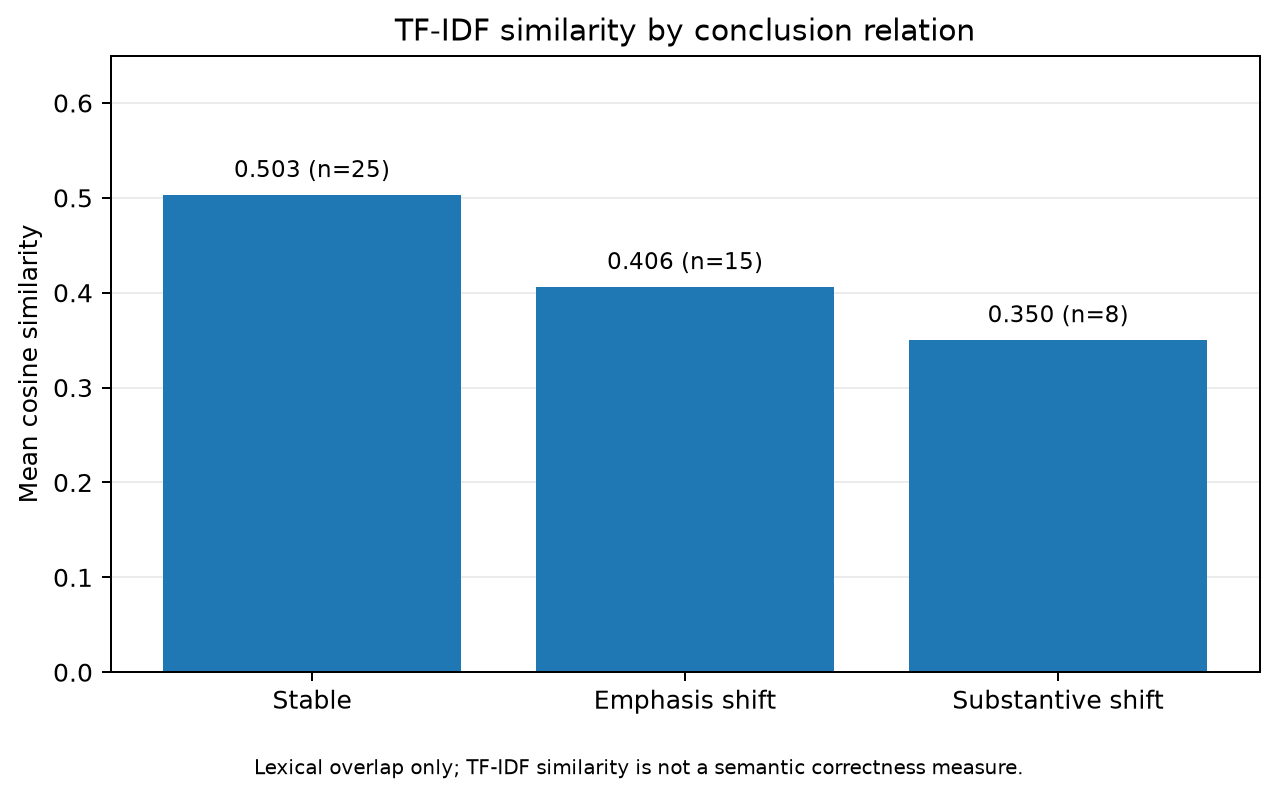
\includegraphics[width=0.88\linewidth]{figures/tfidf_by_conclusion_relation.png}
  \caption{TF--IDF cosine similarity grouped by source-grounded conclusion relation.}
  \label{fig:tfidf}
  \Description{Distribution of TF-IDF cosine similarities grouped by the source-grounded pairwise relation label.}
\end{figure}

\subsection{Qualitative failure cases}
Several outputs illustrate why source-grounded evaluation is needed. For S02, the 0.5B/P0 output introduced extinction risk and identified mammals and reptiles as especially vulnerable, whereas the abstract reported projected species-richness reductions with birds and plants most affected. For S03, the 0.5B/P0 output added Maharashtra and Gujarat, although the study compared Madhya Pradesh, Uttar Pradesh, and Karnataka. For S05, both models' P0 outputs described handwashing after meals, changing the source's measured occasion of handwashing after defecation. In S04, outputs described peer assessment as being used ``in conjunction with'' an online platform, which may conflate the educational intervention with the platform used to conduct the experiment. In S06, the 0.5B/P0 output generalized one inconclusive outcome into broad uncertainty about the intervention despite several statistically significant between-group outcomes. These cases are illustrative rather than an exhaustive failure taxonomy.

\section{Discussion}
The results provide a qualified answer to RQ1. In this run, changing the opening task phrase was associated with changes in generated conclusions, but the changes were not uniform. Just over half of prompt pairs were judged stable, nearly one-third showed emphasis shifts, and one-sixth showed substantive shifts. No contradiction label was assigned. The concentration of substantive shifts in the 0.5B condition suggests a possible difference in robustness between the two tested model sizes, consistent with the broader question of model-size effects discussed in prior prompt-sensitivity research \cite{zhuo2024}. However, this small, single-run comparison cannot establish that increasing parameter count generally reduces prompt sensitivity.

The quality results show that accurate recovery of a broad central finding does not guarantee preservation of its evidential scope. Central-conclusion fidelity was the strongest dimension on average, while scope and qualification fidelity was the weakest. In practical research workflows, that distinction matters: omitting a null result, limitation, conditional threshold, or population boundary can change how a reader interprets a conclusion even if the main direction of the finding remains recognizable. The observed failures in the biodiversity, education, handwashing, and health-coaching abstracts demonstrate different forms of distortion, including invented details, altered measurement conditions, and loss of outcome-specific qualifications.

RQ2 receives a similarly qualified answer. Stable pairs had higher mean lexical similarity than substantive-shift pairs, but the difference is only an association in this small sample. TF--IDF is sensitive to shared vocabulary and may assign high similarity to outputs that retain the same unsupported assertion. It may also assign lower similarity to outputs that express the same conclusion with different wording. Therefore, lexical overlap can be used as a diagnostic comparator, but it should not replace source-grounded assessment of claims, scope, and qualifications.

The adapted pairwise score also needs careful interpretation. The lower value for the 1.5B model indicates less variation in the rubric scores across prompt conditions, not necessarily greater correctness. A model could produce similarly incomplete outputs under all prompts and therefore appear stable under a score-variation metric. For this reason, the study reports absolute source-grounded quality alongside pairwise stability rather than treating stability as a proxy for quality.

The findings support a practical recommendation for LLM-assisted research: evaluate prompt variants using both output-level source fidelity and pairwise conclusion relations. A workflow that reports only lexical similarity or consistency may miss stable but unsupported claims, while a workflow that reports only average quality may conceal cases where the prompt changes the conclusion materially. The two dimensions should be reported together.

\section{Limitations and Threats to Validity}
This study has several limitations. First, the dataset contains only eight purposively selected abstracts and is not representative of scientific literature. Its domain heterogeneity is useful for observing varied failure types but makes the aggregate mean sensitive to the specific source set. Second, abstracts provide less context than full papers; a claim not verifiable from the abstract may be supported elsewhere in the article. Third, the comparison includes two sizes from one model family and does not support generalization to other model families or hosted LLMs.

Fourth, only one greedy generation was produced per source--prompt--model condition. The design therefore measures sensitivity across prompt wordings under a fixed decoding procedure, not stochastic run-to-run variation. Fifth, the three prompt phrases were intended to be meaning-preserving, but perfect semantic equivalence cannot be guaranteed. Sixth, three outputs failed the one-sentence heuristic; they were retained to avoid post hoc editing, but their format deviations may influence interpretability. Seventh, all quality scores and pairwise relation labels were generated through AI-assisted source-grounded assessment. They are not independent human ground truth, and no inter-annotator agreement was measured. Human review of the 48 output assessments and 48 pair labels is required before treating them as final annotations. No statistical-significance tests are reported because the sample is small, purposively selected, and contains one generation per experimental condition.

Finally, the adapted PSS-style score is a study-specific summary of rubric-score differences inspired by ProSA/PSS, not the official PromptSensiScore and not a full reproduction of ProSA. Its numerical values should not be directly compared with published ProSA results.

\section{Conclusion and Future Work}
This controlled comparison examined three paraphrases of a source-only instruction across eight scientific abstracts and two Qwen2.5 model sizes. In the AI-assisted assessment, 25 of 48 prompt pairs were stable, 15 showed emphasis shifts, and eight showed substantive shifts; all eight substantive shifts occurred in the 0.5B condition. The 1.5B model had higher mean source-grounded quality and a lower adapted pairwise score in this sample, while scope and qualification fidelity remained the weakest quality dimension for both models. TF--IDF similarity was higher on average for stable pairs than for substantive-shift pairs, but lexical overlap did not fully determine substantive relation.

These results suggest that prompt wording can affect the content and qualifications of generated scientific conclusions, while also showing that the majority of observed pairwise differences were stable or emphasis-related rather than substantive. The conclusions remain exploratory because the dataset is small and purposive and the annotations are AI-assisted. Future work should add independent human annotation, expand the number and diversity of sources, test additional model families, and repeat generations to estimate stochastic variability. Full-text evidence could also be used to distinguish claims unsupported by an abstract from claims unsupported by the complete paper.

\section*{AI Assistance and Research Provenance}
AI tools were used to assist with experimental code development, debugging, source-grounded assessment, metric computation, visualization, and manuscript preparation. The main outputs were generated by the pinned Qwen2.5 models under the recorded settings. The annotations and relation labels in this paper were generated with AI assistance and have not been independently human-validated. The raw run, exact prompts, model revisions, environment metadata, annotation CSV, pairwise relation CSV, summary metrics, and figures are included in the accompanying reproducibility package. The student author remains responsible for checking the outputs, citations, interpretations, code, and final claims before submission.

\bibliographystyle{ACM-Reference-Format}
\bibliography{second_paper_references}

\end{document}